% Human Action Recognition and Prediction:A Survey
% https://arxiv.org/pdf/1806.11230.pdf 
%

\chapter{Features}
\label{ch:features}
Een belangrijk aspect bij menselijke actieherkenning is het extraheren van bepaalde informatie 
Om menselijke actieherkenning toe te passen is er een omzetting nodig van de ruwe beelden tot een vorm zodat gelijkaardige uitvoeringen van éénzelfde actie door dezelfde structuur kan beschreven worden. Aangezien dat het om menselijke actieherkenning gaat, is het enkel nuttig om informatie over de persoon die de actie uitvoert bij te houden. Een camera die aan het filmen is genereert frames. Men zou voor elke frame een nuttige beschrijving kunnen zoeken zodat enkel informatie overblijft van de persoon zelf. Zo een beschrijving wordt een \textit{feature vector} genoemd. Deze \textit{feature vector} kan verschillende vormen aannemen, maar elke vorm heeft de volgende gelijkenis: de \textit{feature vector} is een rij van getallen waarbij elk getal een ander attribuut beschrijft. Als voorbeeld nemen we skeletdata. De Kinect sensor kan voor elke frame op basis van de ruwe kleuren- en dieptebeelden een skeletbeeld genereren met maximum 25 punten. Elk punt kan geïdentificeerd worden door zijn x, y, en z coördinaten. Per frame kan er dan een \textit{feature vector} $f$ opgebouwd worden met 75 waarden, die de x, y en z beschrijven voor elk van de punten.
$$f =  \begin{pmatrix}
x_1 & y_1&  z_1&  x_2&  y_2&  z_2&  ...&  x_{25} & y_{25}& z_{25}
\end{pmatrix}$$

Dit is slechts één van de vele mogelijke \textit{feature vectors} die kunnen opgesteld worden. Dit hoofdstuk verkent de mogelijkheden van \textit{features} voor zowel kleuren- als dieptebeelden.


\section{Features uit kleurenbeelden}
De extractie van features bij kleurenbeelden kan in twee categorieën onderverdeeld worden: \textit{globale feature extraction} en \textit{lokale feature extraction} \cite{Poppe2010}. Bij een globale aanpak wordt een persoon eerst gelokaliseerd met behulp van \textit{background subtraction} of \textit{tracking} gevolgd door het encoderen van de interesseregio's. Background subtraction kan enkel met statische camera's uitgevoerd worden. Er wordt een referentieframe bijgehouden die enkel statische informatie bevat. Het verschil tussen een nieuwe frame en de referentieframe kan nieuwe informatie opleveren. Deze representatie kan veel informatie bevatten, maar door de nood aan background subtraction of tracking zijn zulke methoden gevoelig aan ruis.

Een lokale aanpak tracht deze problemen te vermijden door eerst lokale interessepunten, in de literatuur \gls{ac:stip} genoemd, te bepalen. Deze interessepunten kunnen zowel het temporale als het ruimtelijke aspect modelleren. Rond deze interessepunten worden patches berekent, afhankelijk van gekozen parameters. De verzameling van zulke patches is de representatie. 
 
feature detectors:
\todo{harris3D \cite{Laptev2005}}
\todo{cuboid \cite{Dollar2005}} 
\todo{Hessian \cite{Willems2008}}
\todo{dense trajectory \cite{Wang2011}}

feature descriptors:
\todo{cuboid descriptor: \cite{Dollar2005}}
\todo{hog/hof \cite{Laptev2005}}
 
\section{Features uit dieptebeelden}
\begin{figure}
	\centering
	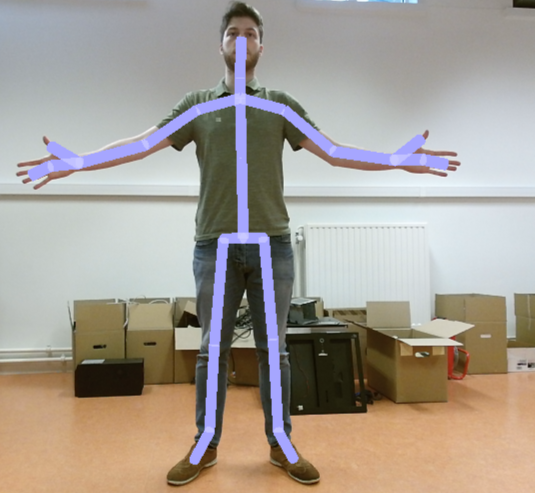
\includegraphics[width=0.5\textwidth]{skeleton_joints}
	\caption{De 25 skeletjoints. De Kinect stelt onder andere de drie-dimensionale coördinaten en de relatieve quaternionen ter beschikking.}
	\label{fig:skeleton_joints}
\end{figure}
De algoritmen die bruikbaar zijn op kleurenbeelden kunnen niet toegepast worden op dieptebeelden. 

Literatuur over feature extraction op dieptebeelden levert vaak algoritmen \cite{Xia2012}, \cite{Wang2012b}, \cite{Yang2012} op die gebruik maken van skeletbeelden gegeneerd met methode \cite{Shotton2011} waarop de skelettracker van de Kinect op gebaseerd is. De skeletbeelden van de Kinect geven de drie-dimensionale coördinaten van 25 punten, \textit{joints} genoemd, die belangrijke kenmerken van het menselijk lichaam voorstellen. Al deze joints worden weergegeven op figuur \ref{fig:skeleton_joints}.

Het gebruik van de Kinect is geen vereiste om actieherkenning met dieptebeelden uit te voeren. \cite{Li2010} stelt elke frame voor als een verzameling van 3D punten, geëxtraheerd uit de silhouetten dat de dieptebeelden geven en maken gebruik van een \gls{ac:hmm} om het temporale aspect te modelleren. \cite{Wang2012a} 

In volgende onderdelen worden een aantal belangrijke feature descriptors beschreven.
\subsection{Histograms of 3D Joints (HOJ3D)}
Het werk van \cite{Xia2012} toont aan hoe een histogram van drie-dimensionale punten aan real-time actieherkenning kan doen. Ze transformeren het skeletbeeld gegenereerd door de Kinect om in bolcoördinaten. Als oorsprong wordt de heup joint genomen. De horizontale referentievector $\mathbf{\alpha}$ wordt parallel met de grond genomen door de oorsprong. De verticale referentievector $\mathbf{\theta}$ staat loodrecht op $\mathbf{\alpha}$ en gaat ook door de oorsprong. De drie-dimensionale ruimte wordt opgesplitst in $84$ deelruimten. Elke joint zal zich dan in één van die 84 deelruimte bevinden. Een histogram wordt opgemaakt door elke joint te wegen in 8 naburige deelruimten via een Gaussische functie:

$$p(X, \mu, \Sigma) = \frac{1}{(2\pi)^{n/2}|\Sigma|^{1/2}}e^{-\frac{1}{2}(X - \mu)^T\Sigma^{-1}(X - \mu)}$$

Hierbij is $\mu$ de mediaanvector en $\Sigma$ de identiteitsmatrix. Voor zowel $\mathbf{\Theta}$ als $\mathbf{\alpha}$ wordt de kansfunctie apart uitgerekend. Stel $\Omega$ de cumulatieve distributiefunctie van de normaalverdeling, dan wordt de kans dat een joint met locatie $(\mu_\alpha, \mu_\theta)$ 


Dit levert de \gls{ac:hoj3d} descriptor op. \todo{nog verder}



\subsection{Covariance Descriptors on 3D Joint Locations (COV3DJ)}
De methode van \cite{Hussein2013} maakt gebruik van covariantiematrices. Een covariantiematrix voor een verzameling van $N$ willekeurige variabelen is een $N \times N$ matrix waarvan de elementen de covariantie bevatten tussen elk paar variabelen. Als $\textbf{X} = (X_1, X_2, ..., X_N)$, een vector met $N$ random variabelen, dan wordt een element $K_{X_{i}X_{j}}$ van de covariantiematrix $K$ gedefinieerd als:

$$K_{X_{i}X_{j}} = E[(X_i - E[X_i])(X_j - E[X_j])]$$

Zo een matrix bevat informatie over de gezamenlijke kans $P(X_j) \cdot P(X_i | X_j)$. Het eerste gebruik van zo een matrix is in het werk van \cite{Tuzel2006} met als doel een regio van een afbeelding te beschrijven.

Elke joint $i$ kan voorgesteld worden door zijn drie-dimensionale coördinaten voor een frame $t$: $p_i^{(t)} = (x_i^{(t)}, y_i^{(t)}, z_i^{(t)})$. De concatenatie van alle joints voor frame $t$ is een vector $\textbf{S}$, met $3K$ elementen: $\textbf{S} = (x_1, ..., x_K,y_1, ..., y_K,z_1, ..., z_K)$, hierbij is $K$ het aantal joints dat beschikbaar is op één frame. Voor $\textbf{S}$ kan nu de covariantiematrix berekent worden, maar de kansverdeling is niet gekend, zodat de steekproefcovariantie wordt gekozen. De resulterende matrix is symmetrisch ten opzichte van de hoofddiagonaal, zodat enkel de bovendriehoek in het geheugen beschikbaar moet zijn. Voor $K = 25$ is het aantal resulterende elementen in de bovendriehoek gelijk aan $2850$. In vergelijking met \cite{Hussein2013} waarbij ze $K = 20$ nemen, is het resultaat $1830$. Vijf extra joints zorgt al voor een toename van 1020 elementen in de matrix.

Deze descriptor, \gls{ac:cov3dj} genoemd, bevat de locaties van de verschillende joints, afhankelijk van elke andere joint tijdens een actie. De temporale informatie wordt beschreven als een hiërarchie van zulke descriptors. Het niveau $l$ duidt de diepte in de hiërarchie aan waarbij $l = 0$ de top van de hiërarchie is. Elk niveau bevat $2^l - 1$ descriptors die elk $\frac{T}{2^l}$ frames bevatten van de sequentie. Voor $l = 1$ zullen er drie descriptors gegenereerd worden die elk $T/2$ frames zullen modelleren waarbij $T$ het totaal aantal frames is. Dit wordt grafisch weergegeven op figuur \ref{fig:temporal_evolution_cov3dj}.

\begin{figure}
	\centering
	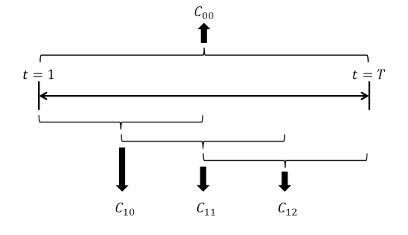
\includegraphics[width=0.5\textwidth]{temporal_evolution_cov3dj}
	\caption{De temporale constructie van de descriptor. $C_{li}$ is de $i$-de descriptor op niveau $l$. }
	\label{fig:temporal_evolution_cov3dj}
	\source{Figuur 2 in \cite{Hussein2013}.}
\end{figure}

Elke descriptor op elk niveau bevat nog steeds hetzelfde aantal elementen ($1830$ voor $K = 20$ of $2850$ voor $K = 25$), zodat de lengte van de totale descriptor nu gelijk is aan het aantal descriptors maal het aantal elementen. Voor $K = 20$ en $K = 25$ bedraagt de lengte van de totale descriptor voor figuur \ref{fig:temporal_evolution_cov3dj} respectievelijk $7320$ en $11\,400$ elementen. 


\subsection{Local Occupancy Pattern (LOP)}
Deze methode \cite{Wang2012b} berekent allereerst de drie-dimensionale afstand van elke joint $i$ tot elke andere joint $j$: $\textbf{p}_{ij} = \textbf{p}_i - \textbf{p}_j$. De feature vector voor elke joint $i$ wordt dan:
$$\textbf{p}_i = \{\textbf{p}_{ij} | i \neq j \}$$

Aanvullend aan deze feature wordt een \gls{ac:lop} gedefinieerd. Deze feature geeft de lokale bezettingsgraad aan; een maat om aan te geven in hoeverre een joint door een ander object gehinderd wordt. Op frame $t$ wordt er een puntenwolk gegenereerd op basis van het dieptebeeld. Voor elke joint $j$ wordt zijn lokale regio gepartitioneerd in een $N_x \times N_y \times N_z$ raster. Elke cel van dit raster bevat $S_x \times S_y \times S_z$ pixels. Voor elke cel $c_{xyz}$ wordt de som van de punten genomen die zich in die cel bevinden. De sigmoïdefunctie $\delta(x) = \frac{1}{1 + e^{-\beta x}}$ wordt toegepast op deze som om zo de feature $o_{xyz}$ te bekomen:

$$o_{xyz} = \delta\bigg(\sum_{q \in c_{xyz}} I_q \bigg)$$


\begin{itemize}
	\item \textbf{Inleiding:} Ze ontwikkelen een manier om intra-klasse variantie op te lossen met dieptebeelden + skeletbeelden via \cite{Shotton2011}. Ze geven ook nieuwe features die voor dieptedata werken. Ze vermelden dat features sensorafhankelijk zijn. Bij kleurenbeelden wordt bijvoorbeeld \gls{ac:stip} \cite{Laptev2003} gebruikt om interessepunten te vinden, en gebruiken \gls{ac:hof} \cite{Laptev2010} of \gls{ac:hog} \cite{Dalal2010}. Voor dieptebeelden werken zo features niet. 
	
	Om het temporale aspect te modelleren worden \gls{ac:hmm} \cite{Lv2006} gebruikt, of \gls{ac:crf} \cite{Han2010}. Andere manier is \gls{ac:dtw} \cite{Muller2006}, maar dat vereist een goede metriek om twee frames te vergelijken. Voor cyclische acties lijkt DTW ook niet goed. Daarom gebruiken zij \gls{ac:ftp}.
	\item \textbf{Methode:}
	\begin{enumerate}
		\item Op basis van dieptedata en 3D joint posities bouwen zij een nieuwe feature \gls{ac:lop} op. Elke 3D joint wordt geassocieerd met zo een \gls{ac:lop}.
		\item Zij gebruiken niet individuele joints, maar gebruiken de relatieve positie. Een joint $i$ heeft 3 (genormaliseerde) coördinaten $p_i(t) = (x_i(t), y_i(t), z_i(t))$ op een frame $t$.
		
		Ze berekenen $\textbf{p}_{ij} = \textbf{p}_i - \textbf{p}_j$, de relatieve positie van een joint $i$ met elke andere joint $j$. Op die manier wordt er voor elke joint $i$ de feature bepaalt:
		
		$$\textbf{p}_i = \{\textbf{p}_{ij} | i \neq j \}$$
		
		Tussen elk paar joints berekenen is overbodig, ze introduceren daarom actionlet mining om enkel de joints te selecteren die nuttig zijn voor de classificatie.
		
		\item De bijkomende feature, \gls{ac:lop} dient om de lokale diepte voor de joints te modelleren. Ze construeren een drie-dimensionale puntenwolk rond een bepaalde joint.
		
		Voor frame $t$ kan voor elke joint $j$ een puntenwolk opgebouwd worden als volgt:
		
		\begin{enumerate}
			\item De lokale regio van $j$ wordt gepartitioneerd in een $N_x \times N_y \times N_z$ grid. Elke bin in de grid heeft  $(S_x, S_y, S_z)$ pixels.
			\item Het aantal punten voor $t$ dat in elke bin $b_{xyz}$ zit wordt geteld. Er wordt een sigmoid normalisatiefunctie toegepast om de feature $o_{xyz}$ te bekomen voor $b_{xyz}$. De \textit{local occupancy information} voor die bin wordt dan:
			
			$$o_{xyz} = \delta(\sum_{q \in bin_{xyz}} I_q)$$
			
			met $I_q = 1$ als er zich een punt bevindt op locatie $q$ en 0 anders en $\sigma(x) = \frac{1}{1 + e^{-\beta x}}$ 
			
			\item Voor elke frame $t$ zijn er twee features: De 3D posities $\textbf{p}_i[t]$ en de LOP features $\textbf{o}_i[t]$. Via \gls{ac:ftp} wordt de temporale dynamiek gemodellerd.
		\end{enumerate} 
	\end{enumerate}
	\item \textbf{Gebruikte datasets:}
	\begin{itemize}
		\item MSRDailyActivity3D Dataset
		\item CMU MoCap Dataset
	\end{itemize}
	\item \textbf{Toekomst:}
	\begin{itemize}
		\item Gebruik van actionlets om meer complexere acties te begrijpen.
	\end{itemize}
\end{itemize}


\subsection{EigenJoints}
Het werk van \cite{Yang2012} introduceert een nieuwe soort joint, de \textit{EigenJoint}. Ze maken gebruik van de drie-dimensionale positieverschillen tussen elk paar van joints, zoals bij \gls{ac:lop}, en extraheren drie features voor elke frame $c$: de \textit{posture feature} $f_{cc}$, de \textit{motion feature} $f_{cp}$ en de \textit{offset feature} $f_{ci}$. Deze drie features worden geconcateneerd om de feature $f_c = (f_{cc}, f_{cp}, f_{ci})$ te bekomen. Deze feature wordt genormaliseerd via \gls{ac:pca} \todo{uitleggen PCA}. Elke frame $i$ bevat $N$ joints: $X_i = \{x_1^i, x_2^i, ..., x_N^i \}$

De \textit{posture feature} beschrijft de statische postuur dat een persoon aanneemt. Voor elke joint wordt de drie-dimensionale afstand berekent tussen elk paar van joints voor de huidige frame $c$:
$$f_{cc} = \{x_i^c - x_j^c | i , j = 1, 2, ..., N; i \neq j\}$$
De dynamiek wordt gemodelleerd met de \textit{motion feature} die de drie-dimensionale afstand berekent tussen elke joint van de huidige frame $c$ met elke andere joint van de vorige frame $p$: 
$$f_{cp} = \{x_i^c - x_j^p | x_i^c \in X_c ; x_j^p \in X_p \}$$

Tot slot wordt nog de \textit{offset feature} gedefinieerd, die de algemeen dynamiek modelleert door de drie-dimensionale afstand te berekenen tussen elke joint van de huidige frame $c$ met elke andere joint van de initiële frame $i$:
$$f_{ci} = \{x_i^c - x_j^i |  x_i^c \in X_c ; x_j^p \in X_i \}$$

De verzameling van deze drie feature vectoren wordt $f_c$ genoemd. Er wordt een lineaire normalisatie uitgevoerd zodat elk attribuut in $f_c$ zich in het bereik $[-1, +1]$ bevindt zodat $f_{norm}$ bekomen wordt. Het aantal dimensies wordt vrij hoog; voor $N = 25$ zorgen $f_{cc}$, $f_{cp}$ en $f_{ci}$ respectievelijk voor $300$, $625$ en $625$ jointbewerkingen op. Elke bewerking genereert drie attributen, $\delta x, \delta y, \delta z$, zodat de totale dimensie van $f_c$ gelijkgesteld moet worden aan $ (300 + 625 + 625) \times 3 = 4650$. In vergelijking met \cite{Yang2012} waarbij ze $N = 20$ gebruiken, is de totale dimensie $2970$.


\subsection{Sequence of the Most Informative Joints (SMIJ)}
Het werk van \cite{Ofli2012} vertrekt van de observatie dat verschillende personen een actie op diverse manieren kunnen uitvoeren, maar dat altijd dezelfde joints gebruikt worden om die actie uit te voeren. Ze berekenen de \textit{relative informativeness} van alle joints in een temporale window tijdens een actie. Een joint kan bijvoorbeeld belangrijk zijn als het de hoogste verandering in hoek heeft. 

Allereerst berekenen ze de hoeken tussen elk paar ledematen die met elkaar verbonden zijn met een joint. De tijdsreeks van deze hoeken wordt als temporale data beschouwd. De vector $\textbf{a}^i$ bevat de tijdsreeks van de hoeken voor joint $i$ voor $T$ frames. Een actie kan dan gezien worden als de verzameling van zulke vectoren:

$$A = [\textbf{a}^1\textbf{a}^2 \cdot\cdot\cdot \textbf{a}^J]$$

Hierbij is $J$ het aantal joints zodat A een $T \times J$ matrix is. Uit A kan het gemiddelde, de variantie en de maximale hoeksnelheid berekent worden voor elke joint. \todo{verder}
	\begin{itemize}
	\item \textbf{Inleiding:} Ze vermelden dat elke persoon een actie op een verschillende manier kan uitvoeren, maar dat zij toch dezelfde joints gebruiken om die actie uit te voeren. Ze berekenen de \textit{relatieve informativeness} van alle joints in een temporale window tijdens een actie. Een joint is bv belangrijk als het de hoogste variantie heeft door de grootste verandering in hoek.
	\item \textbf{Methode:} 
	\begin{enumerate}
		\item Ze berekenen de hoek tussen twee ledematen en gebruiken de tijdsreeks van deze hoeken als motion data. De vector $\textbf{a}^i$ bevat de tijdsreeks van de hoeken voor joint $i$ voor $T$ frames.
		\item Een actie kan dan gezien worden als de verzameling van alle vectoren
		
		$$A = [\textbf{a}^1\; \textbf{a}^2\; ...\; \textbf{a}^J]$$
		
		$J$ is het aantal joints,	dus $A$ is een $T \times J$ matrix.
		
		\item Uit $A$ kan bijvoorbeeld het gemiddelde, variantie en maximale hoeksnelheid berekent worden voor elke joint, hier aangeduid met de operatie $\mathcal{O}$, die een bewerking uitvoert op een vector en een scalaire waarde teruggeeft:
		
		$$\mathcal{O}(\textbf{a}) : \mathcal{R}^{|\textbf{a}|} \mapsto \mathcal{R}$$
		
		\item Een actiesequentie kan nu als feature beschreven worden
		
		$$\textbf{F} = \{\textbf{f}_1, \textbf{f}_2, ..., \textbf{f}_{N_{s}}\}$$
		met
		$$\textbf{f}_k = [\mathcal{O}(\textbf{a}_k^1)\; \mathcal{O}(\textbf{a}_k^2) \; ... \; \mathcal{O}(\textbf{a}_k^J)]$$
		
		Deze worden gesorteerd en zo wordt de SMIJ feature bekomen:
		$$ SMIJ = \{\{ idof(sort(\textbf{f}_k) ,n)\}_{k=1,...,N_s}\}_{n=1,...,N}$$
		In other words, the SMIJ features represent an action sequence by encoding the set of $N$ most informa- tive joints at a specific time instant (by rank-ordering and keeping the top-ranking $N$ joints) as well as the temporal evolution of the set of the most informative joints through- out the action sequence (by preserving the temporal order of
		the top-ranking $N$ joints).
	\end{enumerate}
	\item \textbf{Gebruikte datasets:}
	\begin{itemize}
		\item /
		\item HDM05 database
		\item MSR Action3D dataset
	\end{itemize}
	\item \textbf{Toekomst:}
	\begin{itemize}
		\item {\color{red}Geen. Ze geloven dat hun methode het meest ideale is voor praktische toepassingen.}
	\end{itemize}
\end{itemize}

\subsection{Lie group}
Groepentheorie kan ook gebruikt worden bij actieherkenning. De Lie groep $SO_3$ kan de relatieve drie-dimensionale rotaties tussen elk paar van joints representeren. Deze representatie vormt dan een punt in de Lie groep $SO_3 \times ... \times SO_3$. Een actie is dan een curve in diezelfde Lie groep.
\todo{verder}

Bron \cite{Vemulapalli2014}
\begin{itemize}
	\item \textbf{Inleiding}: Nieuwe representatie voor skelet dat de 3D verhoudingen tussen lichaamsdelen expliciet modelleert, gebruik makend van rotaties en translaties. Zij maken een allereerst een onderscheid tussen \textit{joint-based} en \textit{body-based} actieherkenning
	\begin{itemize}
		\item Joint-based: Het menselijk skelet is gewoon een verzameling van punten. Aantal verschillende methoden:
		\begin{itemize}
			\item Gebruik maken van enkel de joints posities \cite{Hussein2013}, \cite{Lv2006}
			\item Gebruik maken van een assenstelsel \cite{Xia2012}
			\item Paarsgewijze relatieve joint posities \cite{Wang2012b}, \cite{Yang2012}
		\end{itemize}
		
		\item Body-based: Het menselijk skelet is een graaf van joints. \cite{Ofli2012}, \cite{Chaudhry2013}
	\end{itemize}
	
	\item \textbf{Methode:}
	\begin{enumerate}
		\item Een skeletjoint kan met een ander skeletjoint beschreven worden met behulp van rotaties en translaties. M.a.w: de \textit{relatieve geometrie} kan beschreven worden tussen twee punten.
		\item Zulke rotaties en translaties in drie dimensies maken deel uit van de \textit{speciale Euclidische groep} SE(3).
		\item De relatieve geometrie tussen twee joints is een punt in SE(3). Het hele skelet is een punt in $SE(3) \times ... \times SE(3)$.
		\item Acties kunnen nu gerepresenteerd worden door een curve in $SE(3) \times ... \times SE(3)$. Op die curves wordt dan classificatie uitgevoerd.
		\item De groep $SE(3) \times ... \times SE(3)$ is niet vlak, zodat traditionele classificatiemethoden zoals SVM analyse niet direct werken. Daarom wordt de groep eerst gemapt op zijn algebra 
	\end{enumerate}
	\item \textbf{Gebruikte datasets:}
	\begin{itemize}
		\item MSR-Action3D dataset
		\item UTKinect-Action dataset
		\item Florence3D-Action dataset
	\end{itemize}
	\item \textbf{Toekomst:}
	\begin{itemize}
		\item Zij bepalen de relatieve positie tussen elk paar van joints, maar elke actie wordt maar gekarakteriseerd door een specifieke verzameling van joints. Ze zoeken een manier om automatisch te bepalen welke verzameling van joints samen horen tijdens een actie. 
		
		{\color{green}Wordt opgelost in \cite{Wang2012b} met de actionlet mining}
		\item Zij hebben dit ook maar uitgetest op één enkele persoon. Ze willen dit ook uitbreiden naar een multi-persoon model.
	\end{itemize}
\end{itemize}


\subsection{Grassmann manifold}
 Bron \cite{Slama2015}
\begin{itemize}
	\item \textbf{Inleiding:} 
	\item \textbf{Methode:} 
	\begin{enumerate}
		\item De 3D joints worden geëxtraheerd als een tijdreeks. Via het autoregressive and moving average model wordt de dynamiek gemodelleerd. De subspace over de kolommen van de observability matrix is een punt op een grassmann manifold.
		\item Via de 'Riemannian geometry' van dit manifold kan het classificatieprobleem opgelost worden door Control Tangent ruimten te leren die het gemiddelde van elke klasse modelleren.
		
		\item Elke observatie wordt geprojecteerd op alle CTs om een Local Tangent Bandle representatie op te bouwen. Dit dient als input voor een SVM classifier.
	\end{enumerate}
	\item \textbf{Gebruikte datasets:}
	\begin{itemize}
		\item MSRAction3D 
		\item UTKinect
		\item UCFKinect
	\end{itemize}
	\item \textbf{Toekomst:}
	\begin{itemize}
		\item Uitbreiden zodat 'human behaviour recognition' mogelijk is
		\item Extra features gebruiken zodat mens-object interactie kan herkent worden
	\end{itemize}
\end{itemize}

\subsection{Rollende rotaties}

\begin{itemize}	
	\item \textbf{Inleiding:} Ze vermelden ook het verschil tussen joint based en body based: 
	\begin{itemize}
		\item \textbf{Joint based:}
		\begin{itemize}
			\item individuele joints \cite{Gowayyed2013}, \cite{Gu2010}, \cite{Hussein2013}
			\item Pairwise joints \cite{Wang2012b}, \cite{Wang2013}, \cite{Wei2013}, \cite{Yang2012}
			\item Assenstelsel \cite{Xia2012}, \cite{Zhanpeng2013}
		\end{itemize}
		\item  \textbf{Part based:}
		\begin{itemize}
			\item Hoeken: \cite{Ofli2012}, \cite{Ohn-Bar2013}, \cite{JaeyongSung2012}
			\item Bio-inspired : \cite{Chaudhry2013}
			\item relative geometry : \cite{Vemulapalli2014}
		\end{itemize}
	\end{itemize}
	\item \textbf{Uitleg over de groepen:}
	\begin{itemize}
		\item \textbf{$SO_n$}
		
		De speciale orthogonale groep (rotatiegroep) $SO_n$ is een groep gevormd door de verzameling van $n \times n$ matrices $R$ die voldoen aan
		
		$$R^TR = RR^T = I_n$$
		met $|R| = 1$. De elementen van $SO_n$ bewerken punten in $R^n$ via matrix-vector vermenigvuldiging:
		
		$$SO_n \circ R^n \rightarrow R^n, R \circ p = Rp$$
	\end{itemize}
	\item \textbf{Methode:} 
	\begin{enumerate}
		\item Ze representeren een 3D skelet door de relatieve rotaties tussen alle paren van joints. Deze 3D rotaties zijn lid van de Lie group $SO_3$, dus de representatie is een punt in de Lie groep $SO_3 \times ... \times SO_3$. Door de relative 3D rotaties te gebruiken is de representatie schaalinvariant en halveert de feature dimensie, vergeleken met \cite{Vemulapalli2014}.
		\item Een actie is dan een curve in de Lie groep $SO_3 \times ... \times SO_3$. Ze berekenen een verwachte curve, en gebruiken \gls{ac:dtw} om elke andere curve te warpen naar die curve. De \gls{ac:dtw} berekeningen zijn gebaseerd op de kwadratische euclidische afstand in de Lie algebra. Ze hebben het ook geprobeerd met geodisic distance maar da macheert niet. 
		\item Het uitrollen van de Lie group $SO_3 \times ... \times SO_3$ over zijn Lie algebra $so_3 \times ... \times so_3$ samen met elke verwachte vurve. Al de acties worden 'unwrapped' op de Lie algebra. De rolling map voor een gegeven rolling curve kan bekomen worden (theorem 2 in paper)
		\item Elke unwrapped actiecurve wordt een feature vector door alle temporale samples samen te voegen en te classificeren volgens een one-vs-all lineaire SVM classifier.
	\end{enumerate}
	\item \textbf{Gebruikte datasets:}
	\begin{itemize}
		\item FLorence3D dataset
		\item MSRPairs dataset
		\item G3D dataset
	\end{itemize}
	\item \textbf{Toekomst:}
	\begin{itemize}
		\item Rolling map kan voor elke Riemannian manifold gebruikt worden. Zij willen het zeker uitproberen op andere zaken zoals Grassmann manifold en de manifold 
		\item Zij gebruiken enkel skelet features. Indien deze gecombineerd kunnen worden met dieptebeelden zou de accuracy verhoogd kunnen worden.
		\item Zij gebruiken ook de kwadratische afstand. Het zou kunnen geoptimaliseerd worden door 'transported square root vector field' \cite{Su2014} te gebruiken aangezien deze invariant is voor temporale warping.
	\end{itemize}
\end{itemize}



\subsection{3DHoTs}
 Bron \cite{Chen2017}
\begin{itemize}
	\item \textbf{Inleiding:} Een nieuwe low-cost descriptor: 3D histograms of texture (3DHoTs) die features uit dieptebeelden haalt. Dit histogram wordt opgebouwd door de dieptebeelden te projecteren op drie orthogonale cartesische vlakken
	\item \textbf{Methode:} 
	\begin{enumerate}
		\item
	\end{enumerate}
	\item \textbf{Gebruikte datasets:}
	\begin{itemize}
		\item MSRAction3D dataset
		\item MSRGesture3D dataset
		\item UTD-MHAD dataset
		\item MSRActivity3D
	\end{itemize}
	\item \textbf{Toekomst:}
	\begin{itemize}
		\item Uitbreiden zodat het ook werkt voor object herkenning en het opzoeken van images
	\end{itemize}
\end{itemize}



\chapter{Classificatie}
\label{ch:classificatie}
Op het moment dat een feature vector opgebouwd is voor een individuele frame of een verzameling van frames is het actieherkenningprobleem gereduceerd tot een classificatieprobleem. De bekomen feature vector wordt als input aan een classifier gegeven die dan tracht de juiste klasse toe te kennen op basis van de leerverzameling. Een eenvoudige classifier zou een gelijkaardigheidsfunctie $g(\textbf{u}, \textbf{v})$ die nagaat hoe dicht twee \textit{feature vectoren} $\textbf{u}$ en $\textbf{v}$ op elkaar lijken. Dit is echter niet voldoende: 

\section{Leren}
Ongeacht welke classifier gebruikt wordt, moet het eerst leren wat het moet herkennen. Daarom wordt er een leerverzameling $\mathcal{L}$ opgebouwd. Deze verzameling bevat voorbeelden, en in het geval van \textit{supervised learning} ook de klasse (of label) die bij het voorbeeld hoort. Bij actieherkenning bestaat de leerverzameling uit frames en de bijhorende klasse voor elke frame die de corresponderende actie voorstelt. Niet elk voorbeeld uit de leerverzameling wordt gebruikt om te leren: de leerverzameling wordt opgesplitst in een \textit{training set} en een \textit{testing set}. De \textit{training set} wordt gebruikt tijdens de leerfase. In deze fase tracht de classifier optimale parameters te vinden om nieuwe voorbeelden te classificeren. De \textit{testing set} wordt gebruikt na de leerfase om na te gaan hoe goed de classifier scoort en indien nodig wordt de leerfase opnieuw uitgevoerd met andere parameters of \textit{feature} vectoren. Na de leer- en validatiefase komt de gebruiksfase, zodat de classifier kan gebruikt worden. De leerverzameling kan op verschillende manieren opgesplitst worden:
\begin{enumerate}
	\item Er kan door de auteurs van de leerverzameling een voorgedefinieerde splitsing vastgelegd worden. Dit is de minst flexibele methode en wordt ook sterk afgeraden aangezien er een hoge \textit{bias} kan zijn. 
	\item \textit{Leave-$p$-out cross-validation} beschouwt $p$ voorbeelden als de testing set en de overige voorbeelden als training set. Hierbij worden alle mogelijke combinaties uitgevoerd, zodat er $\binom{n}{p}$ keer het model getraind en gevalideert moet worden, met $n$ de lengte van de hele leerverzameling. Het eenvoudigste geval komt voor bij $p = 1$, waardoor er $\binom{n}{1} = n$ validaties zijn, en wordt \textit{leave-one-out cross-validation} genoemd. Deze methode is slechts aangewezen voor $p = 1$ aangezien deze methode  exponentieël gedrag vertoont, waarbij $n^p$ iteraties nodig zijn.
	
	\item \textit{$k-$fold cross-validation} verdeeld de hele leerverzameling in $k$ gelijke groepen. De training set bevat dan $k - 1$ van deze groepen en de testing set bevat de overige groepen. Dit proces wordt $k$ keer herhaald, zodat elk groep zeker eens in de testing set zit. De uitvoeringstijd is hier lineair want in het slechtste geval, voor $k = n$, is de methode exact gelijk aan  \textit{leave-one-out cross-validation}.
\end{enumerate} 

Het grote verschil tussen \textit{$k-$fold cross-validation} en \textit{Leave-$p$-out cross-validation}  is dat de eerste slechts een benadering is van de tweede (voor $k \neq 1$). Bij actieherkenning speelt de uitvoeringstijd een minder grote rol. Een typische leerverzameling die gebruikt wordt bij actieherkenning bestaat uit een aantal acties, die uitgevoerd wordt door verschillende personen. Elke persoon heeft zijn eigen manier om een bepaalde actie, binnen de beperkingen, uit te voeren. Daarom is het nuttig om de leerverzameling op te splitsen door een variant van \textit{Leave-$p$-out cross-validation}, \textit{Leave-one-subject-out cross-validation}. Deze manier verloopt gelijkaardig aan \textit{leave-one-out cross-validation}, maar hier worden de acties van één persoon als testing set beschouwd, terwijl de acties van alle andere personen de training set opmaken.



Voor actieherkenning kunnen drie algemene methoden beschreven worden:
\begin{enumerate}
	\item Classificeren zonder de temporale dimensie expliciet te modelleren, \textit{directe classificatie};
	\item Classificeren waarbij de temporale dimensie wel gemodelleerd wordt, \textit{temporale modellen};
	\item Algemene classificatie zonder de actie te modelleren, \textit{actiedetectie}.
\end{enumerate}


\section{Directe classificatie}
Wanneer het temporale aspect verworpen wordt zijn er maar twee mogelijkheden: alle geobserveerde frames vervatten in één enkele representatie of actieherkenning uitvoeren op elke individuele frame. 

\subsection{$k$-nearest neighbours}

Een voorbeeld van zo een algoritme is $k$-nearest neighbours. Deze methode maakt gebruik van de afstand van de geobserveerde feature vector tot elke andere feature vector uit de leerverzameling. Uit de $k$ dichtste buren wordt dan de klasse genomen die het meest voorkomt. Deze operatie vraagt voor een grote leerverzameling veel rekenkost omdat elke feature vector vergeleken moet worden. De classificatie zal meer tijd vragen naarmate de leerverzameling groter is. 

\subsection{Lineaire classifiers}


\section{Temporale modellen}
\label{subsec:temporale_modellen}
Bij temporale modellen zijn er twee grote klassen te onderscheiden: \textit{generatieve} en \textit{discriminerende} modellen. Een generatief algoritme modelleert hoe een input $x$ wordt gegenereerd om zo een actieklasse $y$ toe te kennen en maakt gebruik van de gezamenlijke kansverdeling $P(x, y) = P(x|y)P(y)$. Een generatief model zal dus de kansverdeling van de leerverzameling modelleren en zal bij een nieuwe observatie \todo{wat zal het doen?}. Een discriminerend model zal de kans $P(y|x)$ direct modelleren zodat een directe mapping van $x$ op $y$ beschikbaar is. De onderliggende kansverdelingen worden dan ook niet berekent.
 Er bestaat een grote discussie over welk van deze twee modellen nu de voorkeur krijgen. Er is aangetoond \cite{Andrew2002} dat discriminerende modellen de voorkeur genieten.

\subsection{Generatieve modellen}
Een markovketen is een speciaal soort automaat die gebruikt kan worden bij het modelleren van temporale processen. Elke markovketen kent een aantal staten $S = \{s_1, ..., s_n\}$ en een $n \times n$ transitiematrix $T$. Deze matrix bevat de waarschijnlijkheid om van één staat naar een andere staat te gaan. Een markovketen gaat uit van twee aassumpties:
\begin{enumerate}
	\item Een verandering van toestand hangt enkel af van de vorige toestand. Dit wordt ook de \textit{Markov eigenschap} genoemd.
	\item De observatie behorend bij een toestand is onafhankelijk van elke andere observatie.
\end{enumerate}
Een markovketen kent ook een uitvoeralfabet $A = \{a_1, ..., a_k\}$ en een $n \times k$ uitvoermatrix $U$. Deze matrix bevat de waarschijnlijkheden dat een bepaalde staat $s_i$ een uitvoer $a_j$ genereerd. 

Een \gls{ac:hmm} is een uitbreiding van een Markov model waarbij de staat van elke toestand nu verborgen is. De toestanden zijn hier de verschillende fasen van een bepaalde actie. Voor een verzameling met $n$ klassen $\Lambda = \lambda^1 ... \lambda^n$ en een verzameling met $k$ observaties $O = \{o_1 ... o_k\}$, moet de juiste klasse $\lambda$ geselecteerd worden die de kans op $P(\lambda | O)$ maximaliseert.

$$\lambda = \arg\max_{\substack{1 \leq i \leq n}} P(O|\lambda^i) $$


\subsection{Discriminerende modellen}
\subsubsection{Conditional Random Fields}
Een \gls{ac:hmm} gaat ervan uit de observaties onafhankelijk zijn van elkaar, wat niet altijd het geval is. Een \gls{ac:crf} is een voorbeeld van een discriminerend model. Een discriminerende classifier houdt rekening met meerdere observaties in de tijd en is geschikt voor de classificatie van een reeks van observaties. Een \gls{ac:crf} gaat ervan uit dat de volgorde van observaties wel degelijk een impact heeft op de betekenis van deze observaties.

\subsubsection{Dynamic Time Warping}
\gls{ac:dtw} is een algoritme dat de gelijkenis tussen twee sequenties bestudeerd, die verschillend kunnen zijn in snelheid. In actieherkenning lost dit het probleem van verschillen in actiesnelheid op. Een persoon die trager of sneller zwaait dan een persoon in de leerverzameling, kan via \gls{ac:dtw} toch herkent worden. Veronderstel twee verzamelingen van feature vectoren $X = \{x_1, x_2, ... x_N\}$ en $Y = \{y_1, y_2, ..., y_M\}$, een kostfunctie $c(x, y)$ die de kost bepaald tussen twee feature vectoren en $p = \{p_1, ..., p_L\}$ met $p_l = (n_l, m_l)$  

Een \gls{ac:dtw} heeft bepaalde restricties:
\begin{itemize}
	\item $p_1 = (1, 1)$ en $p_L = (N, M)$.
	\item $n_1 \leq n_2 \leq ... \leq n_L$ en $m_1 \leq m_2 \leq ... \leq m_L$.
\end{itemize}


\section{Key frames}
In plaats van elke frame te classificeren, zou een actie kunnen voorgesteld worden door \textit{key frames}. Dit is een selectie van frames die een actie voldoende kunnen voorstellen zodanig dat verschillende acties nog steeds onderscheidbaar zijn en variaties van dezelfde actie hetzelfde gelabeld worden. In de literatuur bestaan er diverse manieren om zulke key frames te bepalen. De methode van \cite{Suolan2017} berekent een verschil op basis van de joints die de Kinect beschikbaar stelt. De methode van \cite{Carlsson2001} maakt gebruik van randdetectie om silhouette te bekommen en zoekt een match tussen voorgedefinieerde silhouetten die een key frame van een actie voorstelt. Andere methoden maken ook gebruik van voorgedefinieerde exemplaren \cite{Weinland2008a}, \cite{Fathi2007},



